\section{Introduction}
\label{sec:intro}

The text on which large language models (LLMs) are trained increasingly contains their own outputs.
As synthetic content proliferates across the web, a recursive loop emerges: models trained on web corpora ingest text generated by earlier models, and their outputs feed into the next generation's training data \cite{shumailov2024_nature,alemohammad2024_mad}.
This model$\to$data$\to$model cycle is no longer hypothetical; it is already occurring in the wild. Yet whether the recursive generation depth of a text can be estimated from its statistical properties remains unstudied, a question that matters because first-generation synthetic text may be benign or even beneficial for training, while deeply recursive text drives the distributional collapse that degrades model quality \cite{dohmatob2024_tale_of_tails}.
We focus on the 1--1.5B parameter regime under \emph{controlled full-replacement chains}, where each generation fully replaces the prior training set, isolating the depth variable. Real-world contamination involves partial mixing at unknown proportions; full replacement provides an upper bound on depth signal strength (\S\ref{sec:discussion}).

Existing tools address adjacent but distinct problems.
Binary detectors \cite{binoculars2024,fast_detectgpt2024,diveye2026} collapse all depths $d \geq 1$ into a single category, a limitation we confirm empirically: their pairwise d1-vs-d2 AUC collapses to chance level (\S\ref{sec:gen:baselines}); watermarking \cite{kirchenbauer2023_watermark} requires proactive embedding.
The model collapse literature \cite{shumailov2024_nature,dohmatob2024_tale_of_tails} assumes depth is known a priori; \citet{drayson2025_detection_prevents_collapse} filter synthetic data via binary detection without distinguishing depths.
No existing method estimates the ordinal recursive generation depth of a text passage from its content alone (Figure~\ref{fig:problem}).

We find that recursive generation leaves quantifiable statistical fingerprints in text, and these fingerprints are \textbf{consistent in direction but scale-dependent in magnitude} across the three model families and three decoding strategies studied.
Specifically, the perplexity tail feature family---upper quantiles and kurtosis of the per-token perplexity distribution (\S\ref{sec:method:features})---and surprisal variance emerge as dominant depth indicators, with group-level dominance robust across all 9 model--strategy configurations and three importance measures.
Our contribution centers on task formalization and systematic empirical characterization; the convergence of four classifiers within 0.8\,pp (\S\ref{sec:gen:baselines}) confirms that signal resides in feature design, not classifier architecture.
We formalize recursive generation depth estimation as ordinal classification and find that a lightweight pipeline suffices: compute 19 reference-model statistical features (effective dimensionality ${\approx}$4--5 due to multicollinearity; \S\ref{sec:atlas:features}) and classify with a Random Forest (RF) into $K{+}1$ depth classes.
To characterize how recursive generation reshapes these features, we construct the \emph{Depth Degradation Atlas}: a $3 \times 3$ grid of model families $\times$ decoding strategies spanning 4 depths (180K cell-instances).
The atlas reveals strategy-dependent degradation trajectories; we introduce \emph{Effective Discriminable Depth} (EDD) to quantify how far into the recursion chain adjacent depths remain distinguishable.

\begin{figure*}[t]
\centering
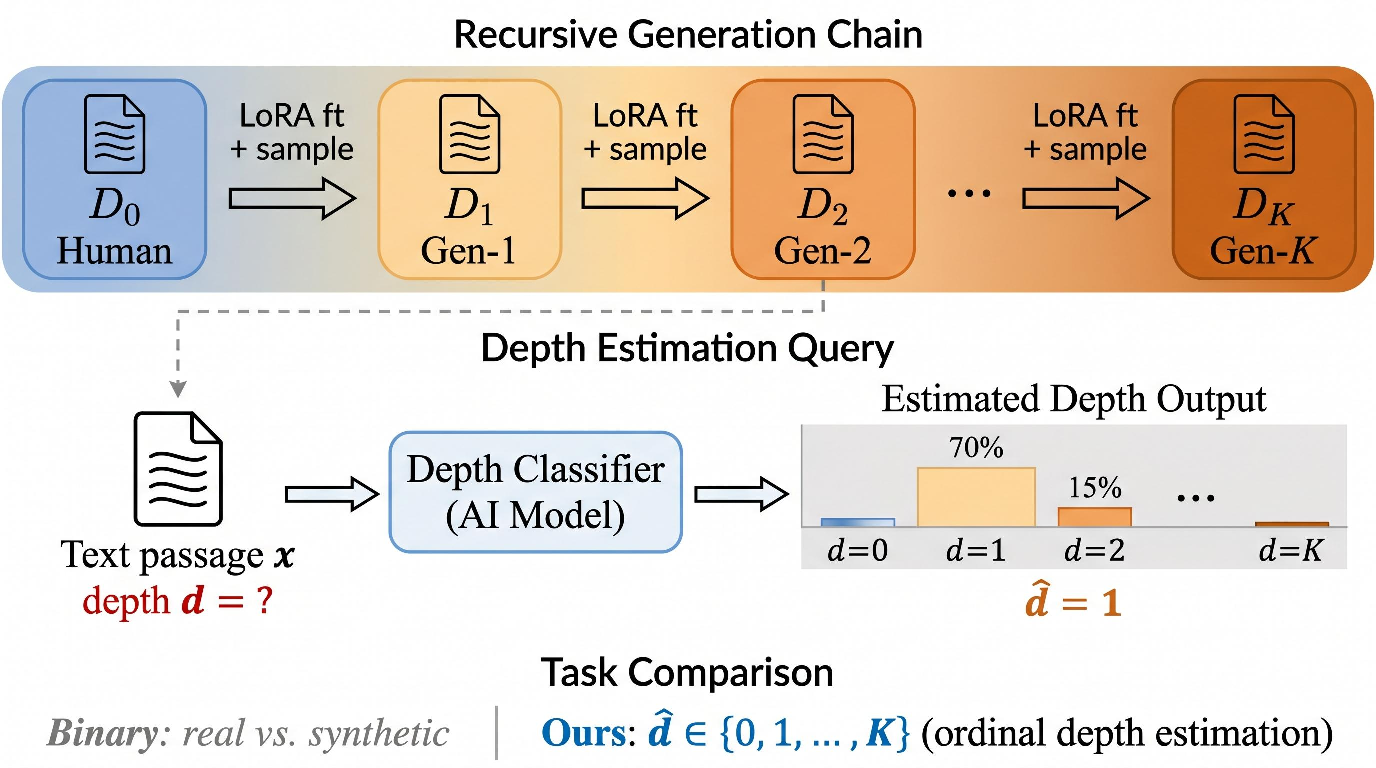
\includegraphics[width=\textwidth]{figures/fig_problem_illustration.pdf}
\caption{Recursive generation depth estimation. A seed corpus $\mathcal{D}_0$ feeds a Low-Rank Adaptation (LoRA) finetuning--sampling loop producing successively deeper corpora. Given a passage~$x$, the task is to estimate its ordinal depth~$d$.}
\label{fig:problem}
\end{figure*}
Our contributions are:
\begin{itemize}[nosep,leftmargin=*]
    \item \textbf{Task formalization and metric.} We define recursive generation depth estimation as ordinal classification, introduce the \emph{Effective Discriminable Depth} (EDD) metric, and construct a 180K cell-instance benchmark ($3$ model families $\times$ $3$ decoding strategies $\times$ $4$ depths; 140K unique passages).

    \item \textbf{Depth Degradation Atlas.} The perplexity tail feature family and surprisal variance jointly dominate depth discrimination across all 9 cells; $\mathrm{EDD}_{0.70}{=}3$ in 8/9 cells (4 under nucleus depth extension), validated by 5-class extension (71--81\%); feature group ablation confirms perplexity tail dominance (76.6\% alone vs.\ 78.4\% full set).

    \item \textbf{Partial-mixing validation.} Under 25--50\% synthetic mixing, $\mathrm{EDD}_{0.70}{=}3$ is preserved in 5/6 cells with $-$8--15\,pp accuracy attenuation.

    \item \textbf{Generalization boundaries.} Within the tested 1--1.5B regime, cross-model transfer reaches 66.4\% and cross-domain (arXiv) 74.1\%; at 14B, cross-reference $\mathrm{EDD}_{0.70}{=}2$; cross-strategy (d1--d3: 45.9\%) is a boundary condition, partially recovered by two-stage routing ($+$11.5\,pp).
\end{itemize}